%保存为UTF-8编码格式
%用xelatex编译
 
\documentclass[UTF8,a4paper,11pt]{ctexart}
\usepackage[left=2.5cm, right=2.5cm, top=2cm, bottom=2cm]{geometry} %页边距
\CTEXsetup[format={\Large\bfseries}]{section} %设置章标题字号为Large,居左
%\CTEXsetup[number={\chinese{section}}]{section}
%\CTEXsetup[name={(,)}]{subsection}
%\CTEXsetup[number={\chinese{subsection}}]{subsection}
%\CTEXsetup[name={(,)}]{subsubsection}
%\CTEXsetup[number=\arabic{subsubsection}]{subsubsection}  %以上四行为各级标题样式设置,可根据需要做修改
 
\linespread{1} %设置全文行间距
 
 
%\usepackage[english]{babel}
%\usepackage{float}     %放弃美学排版图表
\usepackage{fontspec}   %修改字体
\usepackage{amsmath, amsfonts, amssymb} % 数学公式相关宏包
\usepackage{color}      % color content
\usepackage{graphicx}   % 导入图片
\usepackage{subfigure}  % 并排子图
\usepackage{url}        % 超链接
\usepackage{bm}         % 加粗部分公式,比如\bm{aaa}aaa
\usepackage{multirow}
\usepackage{booktabs}
\usepackage{epstopdf}
\usepackage{epsfig}
\usepackage{longtable}  %长表格
\usepackage{supertabular}%跨页表格
\usepackage{algorithm}
\usepackage{algorithmic}
\usepackage{changepage}
\usepackage{caption}
\usepackage[dvipsnames]{xcolor} % 更全的色系
\usepackage{listings} % 排代码用的宏包

\definecolor{mygreen}{rgb}{0.0, 0.5, 0.0}


% 用来设置附录中代码的样式
\lstset{
	basicstyle          =   \sffamily,          % 基本代码风格
	keywordstyle        =   \bfseries,          % 关键字风格
	commentstyle        =   \rmfamily\itshape,  % 注释的风格,斜体
	stringstyle         =   \ttfamily,  % 字符串风格
	flexiblecolumns,                % 别问为什么,加上这个
	numbers             =   left,   % 行号的位置在左边
	showspaces          =   false,  % 是否显示空格,显示了有点乱,所以不现实了
	numberstyle         =   \zihao{-5}\ttfamily,    % 行号的样式,小五号,tt等宽字体
	showstringspaces    =   false,
	captionpos          =   t,      % 这段代码的名字所呈现的位置,t指的是top上面
	frame               =   lrtb,   % 显示边框
}

\lstdefinestyle{Python}{
	language        =   Python, % 语言选Python
	basicstyle      =   \zihao{-5}\ttfamily,
	numberstyle     =   \zihao{-5}\ttfamily,
	keywordstyle    =   \color{blue},
	keywordstyle    =   [2] \color{teal},
	stringstyle     =   \color{magenta},
	commentstyle    =   \color{red}\ttfamily,
	breaklines      =   true,   % 自动换行,建议不要写太长的行
	columns         =   fixed,  % 如果不加这一句,字间距就不固定,很丑,必须加
	basewidth       =   0.5em,
}

\lstset{
	language = matlab,
	backgroundcolor = \color{white}, % 背景色:淡黄
	basicstyle = \small\ttfamily, % 基本样式 + 小号字体
	rulesepcolor= \color{white}, % 代码块边框颜色
	breaklines = true, % 代码过长则换行
	numbers = left, % 行号在左侧显示
	numberstyle = \small, % 行号字体
	keywordstyle = \color{blue}, % 关键字颜色
	commentstyle =\color{mygreen}, % 注释颜色
	stringstyle = \color{purple}, % 字符串颜色
	frame = shadowbox, % 用(带影子效果)方框框住代码块
	showspaces = false, % 不显示空格
	columns = fixed, % 字间距固定
	%escapeinside={} % 特殊自定分隔符:
	morekeywords = {as}, % 自加新的关键字(必须前后都是空格)
	deletendkeywords = {compile} % 删除内定关键字;删除错误标记的关键字用deletekeywords删!
}
 
%%%%%%%%%%%%%%%%%%%%%%%
% -- text font --
% compile using Xelatex
%%%%%%%%%%%%%%%%%%%%%%%
% -- 中文字体 --
%\setCJKmainfont{Microsoft YaHei}  % 微软雅黑
%\setCJKmainfont{YouYuan}  % 幼圆
%\setCJKmainfont{NSimSun}  % 新宋体
%\setCJKmainfont{KaiTi}    % 楷体
\setCJKmainfont{SimSun}   % 宋体
%\setCJKmainfont{SimHei}   % 黑体
 
% -- 英文字体 --
\setmainfont{Times New Roman}
%\setmainfont{DejaVu Sans}
%\setmainfont{Latin Modern Mono}
%\setmainfont{Consolas}
%
%
\renewcommand{\algorithmicrequire}{ \textbf{Input:}}     % use Input in the format of Algorithm
\renewcommand{\algorithmicensure}{ \textbf{Initialize:}} % use Initialize in the format of Algorithm
\renewcommand{\algorithmicreturn}{ \textbf{Output:}}     % use Output in the format of Algorithm
\newcommand{\xiaosi}{\fontsize{12pt}{\baselineskip}}     %\xiaosi代替设置12pt字号命令,不加\selectfont,行间距设置无效
\newcommand{\wuhao}{\fontsize{10.5pt}{10.5pt}\selectfont}
 
\usepackage{fancyhdr} %设置全文页眉、页脚的格式
\pagestyle{fancy}
\lhead{}           %页眉左边设为空
\chead{}           %页眉中间
\rhead{}           %页眉右边
%\rhead{\includegraphics[width=1.2cm]{1.eps}}  %页眉右侧放置logo
\lfoot{}          %页脚左边
\cfoot{\thepage}  %页脚中间
\rfoot{}          %页脚右边
 
 
%%%%%%%%%%%%%%%%%%%%%%%
%  设置水印
%%%%%%%%%%%%%%%%%%%%%%%
%\usepackage{draftwatermark}         % 所有页加水印
%\usepackage[firstpage]{draftwatermark} % 只有第一页加水印
% \SetWatermarkText{Water-Mark}           % 设置水印内容
% \SetWatermarkText{\includegraphics{fig/ZJDX-WaterMark.eps}}         % 设置水印logo
% \SetWatermarkLightness{0.9}             % 设置水印透明度 0-1
% \SetWatermarkScale{1}                   % 设置水印大小 0-1
 
\usepackage{hyperref} %bookmarks
\hypersetup{colorlinks, bookmarks, unicode} %unicode
 
 
 
\title{\textbf{\Large{编程作业四报告}}}
\author{涂宇清}
\date{522030910152}
 
 
 
\begin{document}
 
\maketitle
%\tableofcontents
\setcounter{page}{1}        %从下面开始编页,页脚格式为导言部分设置的格式
 
 
\section{读取乐曲,并绘制其时域波形图和STFT时频图}

\begin{lstlisting}[language=matlab]
[audio, Fs] = audioread([filename, '.wav']);
spectrogram(audio, window, noverlap, nfft, Fs, 'yaxis');
\end{lstlisting}

\begin{figure}[H]   %*表示可跨栏,如果不需要可去掉
    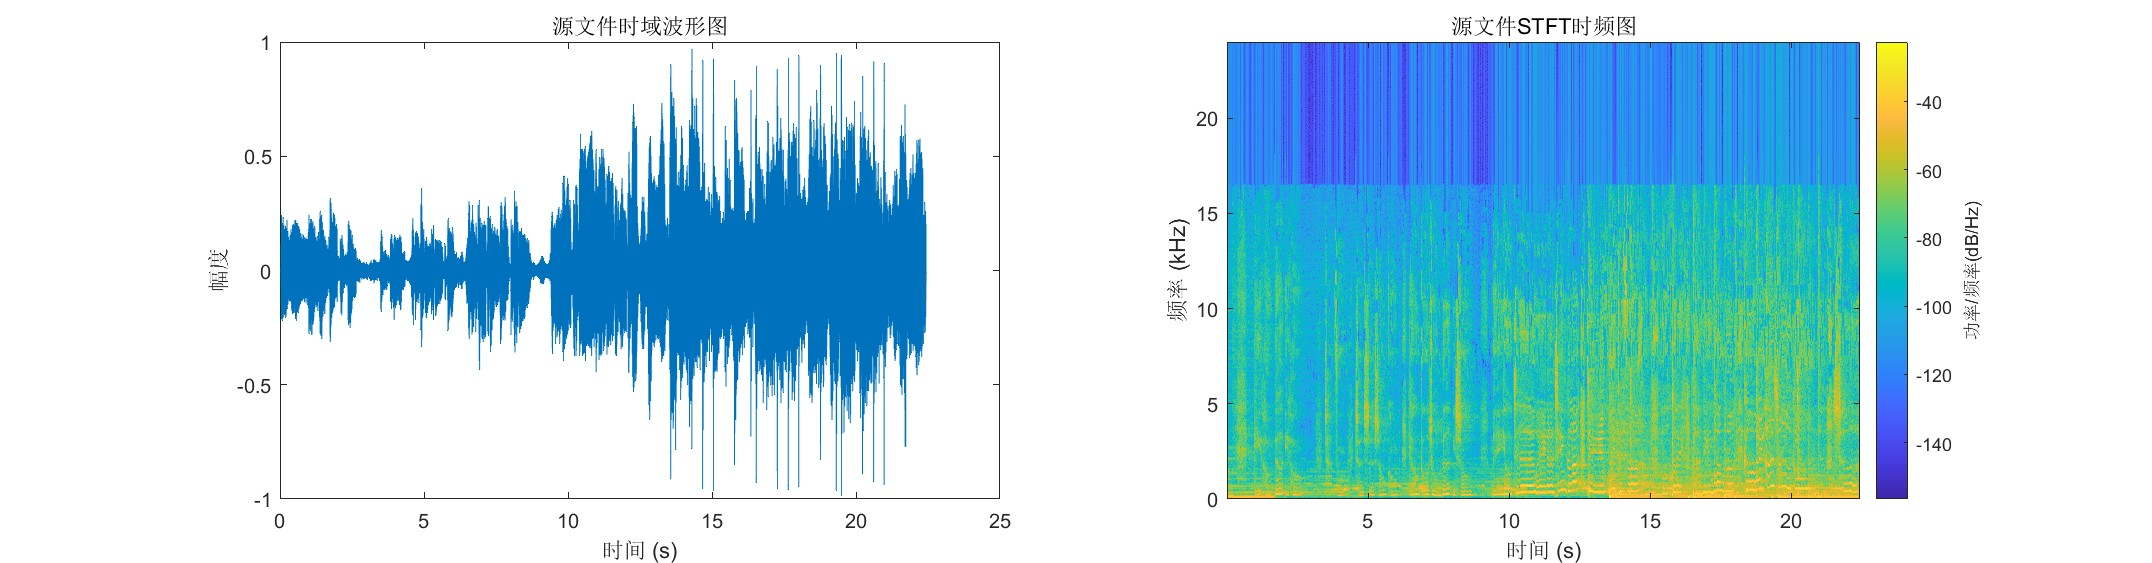
\includegraphics[width=\linewidth]{PA4_1.jpg}
\end{figure}

\section{对乐曲进行下采样,并绘制其时域波形图和STFT时频图}
\begin{lstlisting}[language=matlab]
% 分别以5kHz、10kHz、15kHz的采样率对乐曲进行下采样
resampled_audio_5 = resample(audio, 5e3, Fs);
resampled_audio_10 = resample(audio, 10e3, Fs);
resampled_audio_15 = resample(audio, 15e3, Fs);
\end{lstlisting}

\begin{figure}[H]   %*表示可跨栏,如果不需要可去掉
    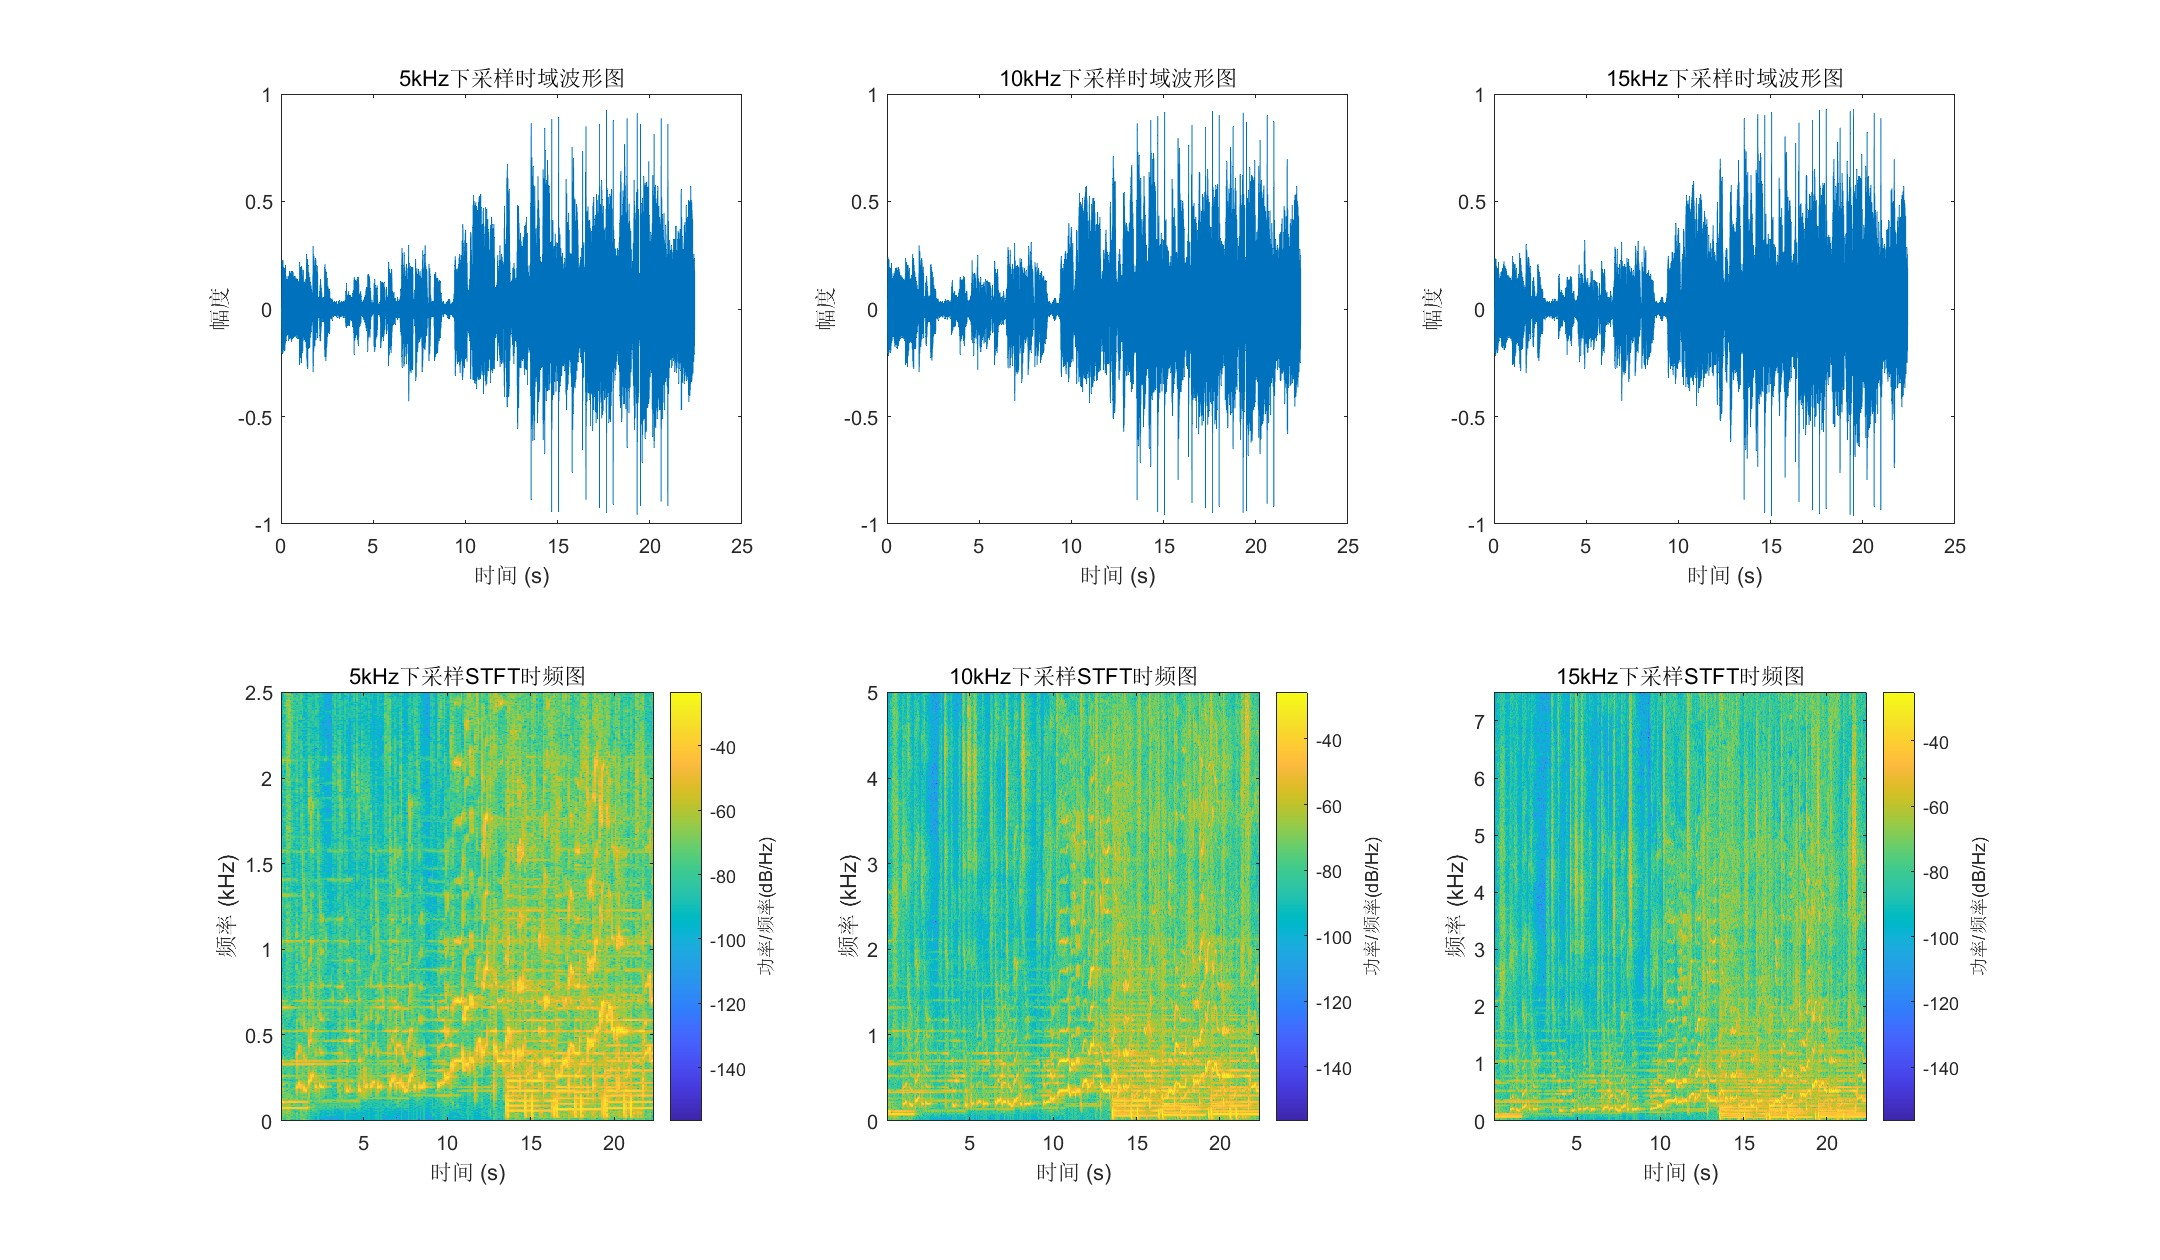
\includegraphics[width=\linewidth]{PA4_2.jpg}
\end{figure}

\section{对下采样后的乐曲进行插值恢复,绘制其时域波形图和STFT时频图并与原乐曲进行对比}

\begin{lstlisting}[language=matlab]
interpolated_audio_5 = resample(resampled_audio_5, Fs, 5e3);
interpolated_audio_10 = resample(resampled_audio_10, Fs, 10e3);
interpolated_audio_15 = resample(resampled_audio_15, Fs, 15e3);
\end{lstlisting}

\begin{figure}[H]   %*表示可跨栏,如果不需要可去掉
    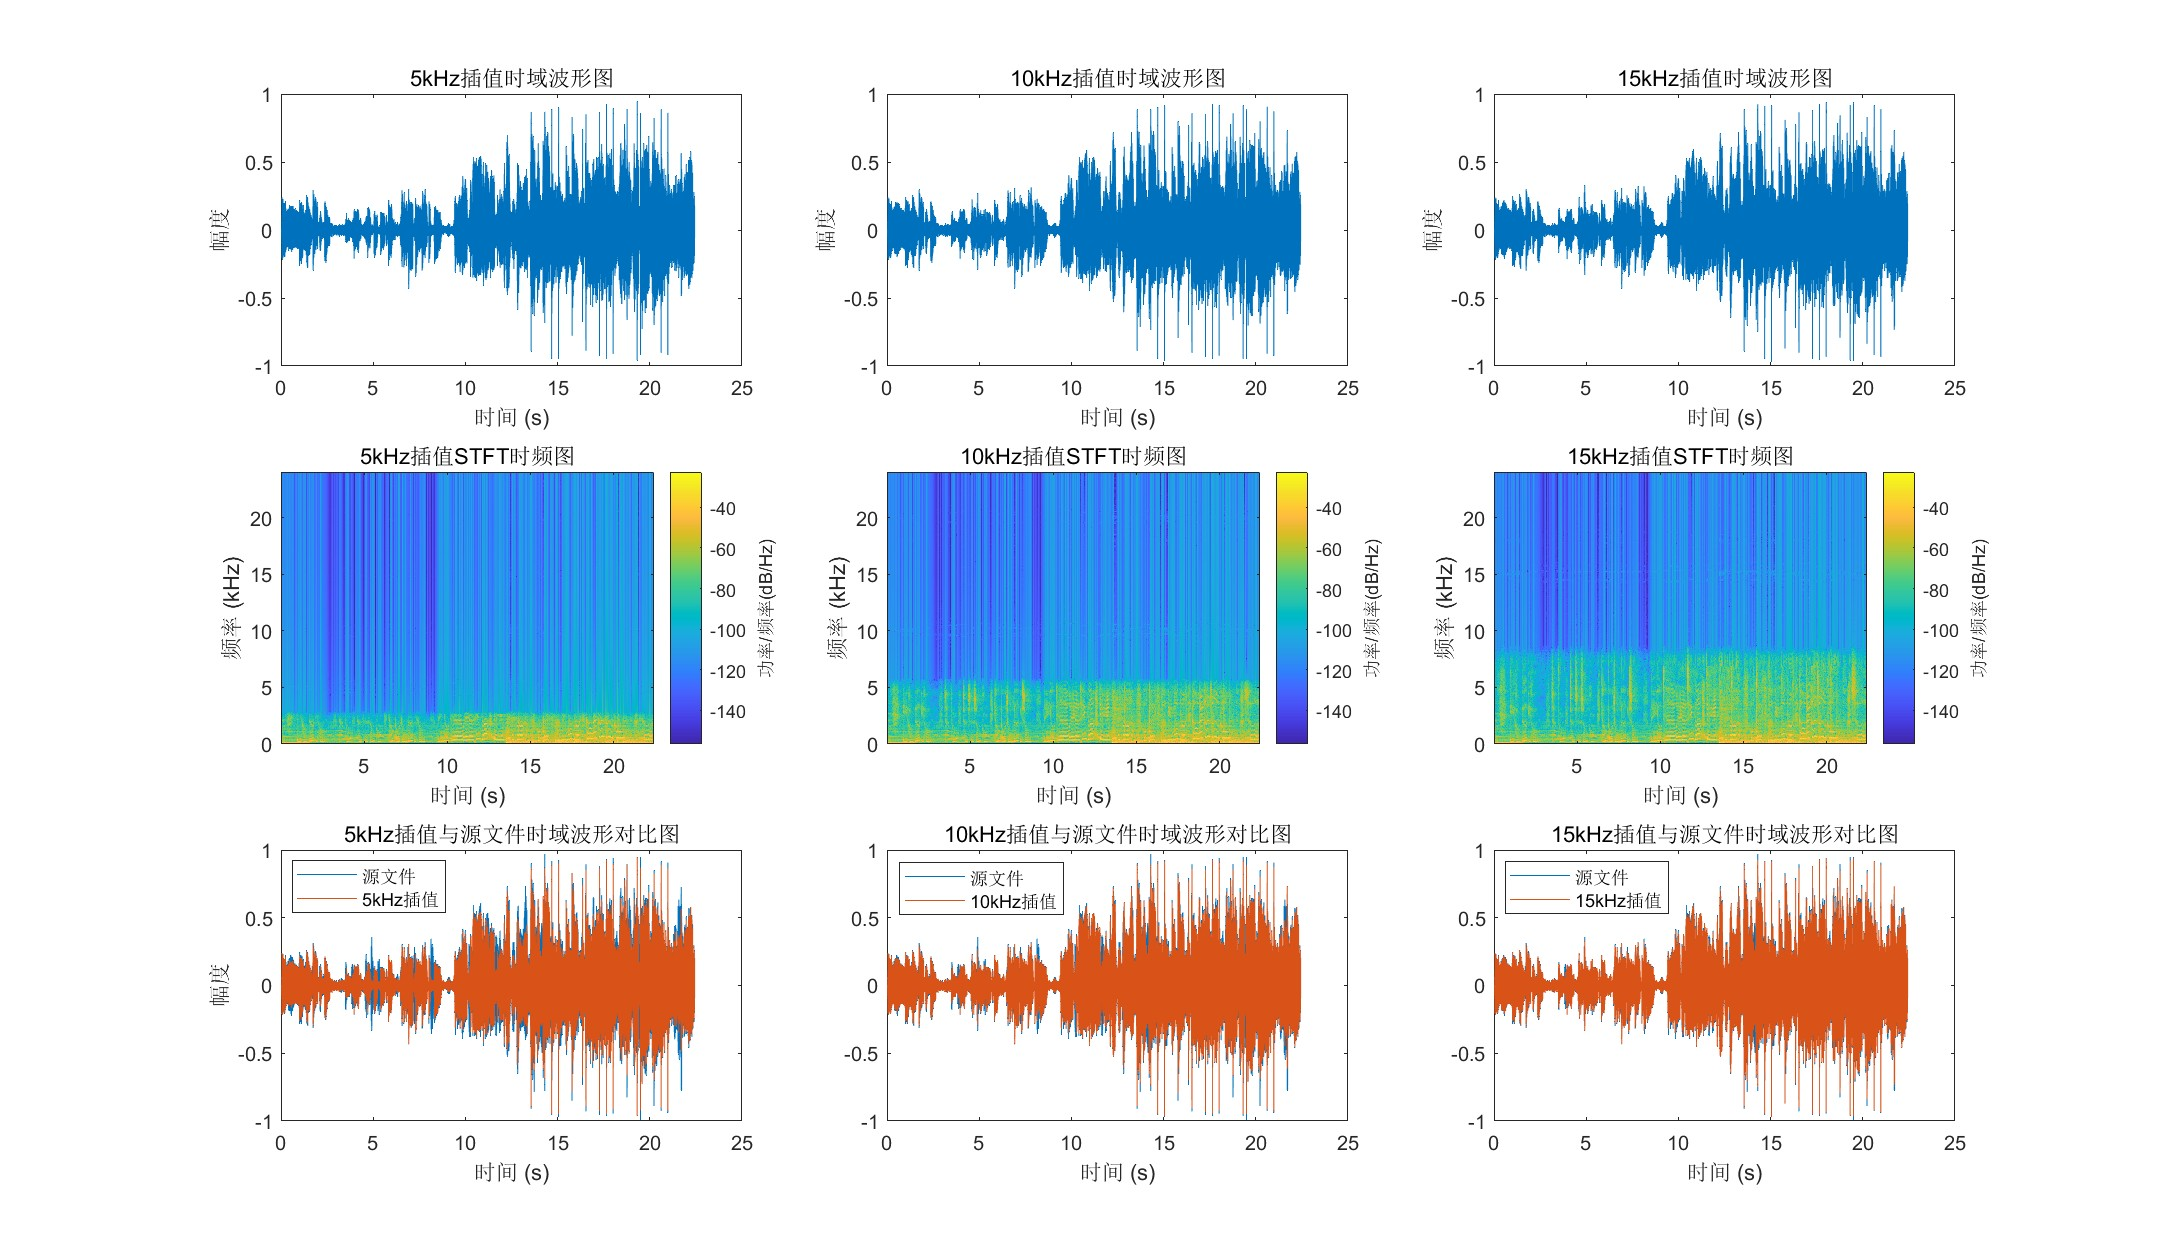
\includegraphics[width=\linewidth]{PA4_3.jpg}
\end{figure}

由对比图可以看出,采样率5kHz的插值恢复效果较差,与原乐曲有较大差距;采样率10kHz的插值恢复效果较好,与原乐曲重合度较高;而采样率15kHz的插值恢复效果最好,与原乐曲几乎完全重合。由此可得,随着采样率的增加,原乐曲损失的信息就越少,插值恢复的效果就越好。

\section{设计一个作用为清晰人声的均衡器,对乐曲进行处理}
\begin{lstlisting}
% 定义窗口参数
win = hamming(128);
overlap = length(win)/2;
nfft = length(win);
% 进行STFT
[S, f, t] = stft(audio, Fs, "Window",win, "OverlapLength",overlap, "FFTLength",nfft);
% 增强人声、削弱乐器
S((f > 5e2) & (f < 8e3), :) = S((f > 5e2) & (f < 8e3), :) * 100;
S((f > 0) & (f < 5e2), :) = S((f > 0) & (f < 5e2), :) * 0.01;
S((f > 8e3) & (f < 24e3), :) = S((f > 8e3) & (f < 24e3), :) * 0.01;
% 进行逆STFT
audio_mod = istft(S, Fs, "OverlapLength",overlap, "FFTLength",nfft);
audio_mod = real(audio_mod);    % 去除虚数部分
normalized_audio = audio_mod / max(abs(audio_mod)); % 归一化,防止失真
\end{lstlisting}

该均衡器通过对人声频率段(500-8kHz)添加20dB的增益,对乐器频率段(0-500Hz,8k-24kHz)添加-20dB的增益,增加了人声与乐器的对比度,使得人声更加清晰。

\end{document}
